% !TEX root = ../Dissertation.tex
%===================================================================================================

\chapter{Materials and Methods}



\section{Mice}
\label{methods:mice}

NOD, NOD.$\mu$MT\textsuperscript{-/-}, NOD-RAG2p-GFP, NOD.$\mu$MT\textsuperscript{-/-}-RAG2p-GFP and C57BL/6 (B6) mice were used.

NOD.$\mu$MT\textsuperscript{-/-} (hereafter referred to as NOD KO) mice are deficient in B cells and have been described elsewhere \citep{Serreze1996}.
They have a mutation in their IgM heavy chain which prevents heavy chain rearrangement and subsequent progression from the pro B cell stage to the pre B cell stage.
This block in development results in an inability to produce B cells.

RAG2p-GFP reporter mice on a FVB background have also been described elsewhere \citep{Yu1999}.
RAG2p-GFP reporter mice express green fluorescent protein (GFP) under the control of the RAG promoter so that when RAG is expressed, so is GFP.
When RAG transcription is deactivated, so is GFP transcription.
However, the protein decays over time with a half life of ~56 hours \citep{McCaughtry2007}, meaning that GFP\textsuperscript{+} cells can be seen even after RAG deactivation.

For use in this project, FVB-RAG2p-GFP mice were backcrossed 12 generations (n12) to the NOD mouse to produce NOD-RAG2p-GFP reporter mice (hereafter referred to as NOD-RAG-GFP mice).

NOD.$\mu$MT\textsuperscript{-/-}-RAG2p-GFP reporter mice (hereafter referred to as NOD KO-RAG-GFP mice) were also used in this project.
For this, n12 NOD-RAG2p-GFP mice were crossed with NOD.$\mu$MT\textsuperscript{-/-} mice.
Heterozygous progeny were then crossed back to NOD.$\mu$MT\textsuperscript{-/-} mice.
Mouse genotypes were determined by bleeding and subsequent flow cytometry to look for GFP presence and B cell absence.

All mice were housed in specific-pathogen-free barrier conditions at York University Biological Services Facility. 
All experimental procedures were conducted under U.K. Government Home Office guidelines.
For mouse studies, investigations were carried out double or single blind, as stated in results, following ARRIVE guidelines \citep{Arriveguidelines}





\section{Cell preparation}
\label{sec:cellprep}

\subsection{Preparation from frozen tissue}

Frozen cells defrosted quickly and transferred to 5 mL phosphate buffered saline (PBS) supplemented with 0.5\% bovine serum albumin (BSA) (hereafter referred to as 0.5\% PBS/BSA).
Samples centrifuged for 3 minutes at 1200 revolutions per minute (rpm), supernatant discarded and cells resuspended in 1 mL 0.5\% PBS/BSA.
Samples centrifuged again as before then resuspended in 2 mL 0.5\% PBS/BSA and put in incubator at 37 \textdegree C for 2 hours.
Samples then centrifuged as before, supernatant discarded and cells resuspended as appropriate for subsequent procedure.

\subsection{Preparation from fresh tissue}
Bone marrow tissue was obtained by flushing of femur and tibia of mouse with 1 x PBS.
Thymi and spleens were homogenised using a seive and syringe plunger.
Suspensions centrifuged for 3 minutes at 1200 rpm to pellet cells then supernatant discarded.
Cells requiring red blood cell lysis were then resuspended in 1 mL of water for 6 seconds followed by 1 mL of 2 x PBS to neutralise toxicity of water.
Lysed samples then centrifuged as before, supernatant discarded and resuspended as appropriate for subsequent procedure.

\section{Flow cytometry}

Single cell suspensions prepared as in \cref{sec:cellprep}.
Samples treated with 1:300 dilution of anti-CD16/32 antibody and incubated for at least 10 minutes at 4 \textdegree C.
This was carried out to block Fc receptors in an attempt to avoid non specific antibody binding in subsequent staining steps.
Samples then stained using appropriate fluorescently labelled antibodies and incubated for 25 minutes at 4 \textdegree C in the dark.
Antibodies (from eBioscience or BD Pharmingen) were used at 1:300 dilution, apart from CD4 and CD8 which were used at 1:800. 
Samples washed in 3 mL PBS and centrifuged for 3 minutes at 1200rpm, supernatant discarded then cells resuspended in 500 $\mu$L of PBS to run on FACS machine.

If biotin/streptavidin antibodies used, then a second round of staining and washing was carried out, in order to add the fluorescently labelled streptavidin at 1:800 dilution.

Data was acquired on a Dako Cyan using Summit software and analysed using FlowJo software.

Antibody clones and suppliers are shown in \cref{fig:antibodyclones}. \todo{Check purified antibody clones, CD25, SA and other CD8 antibodies}

\begin{table}
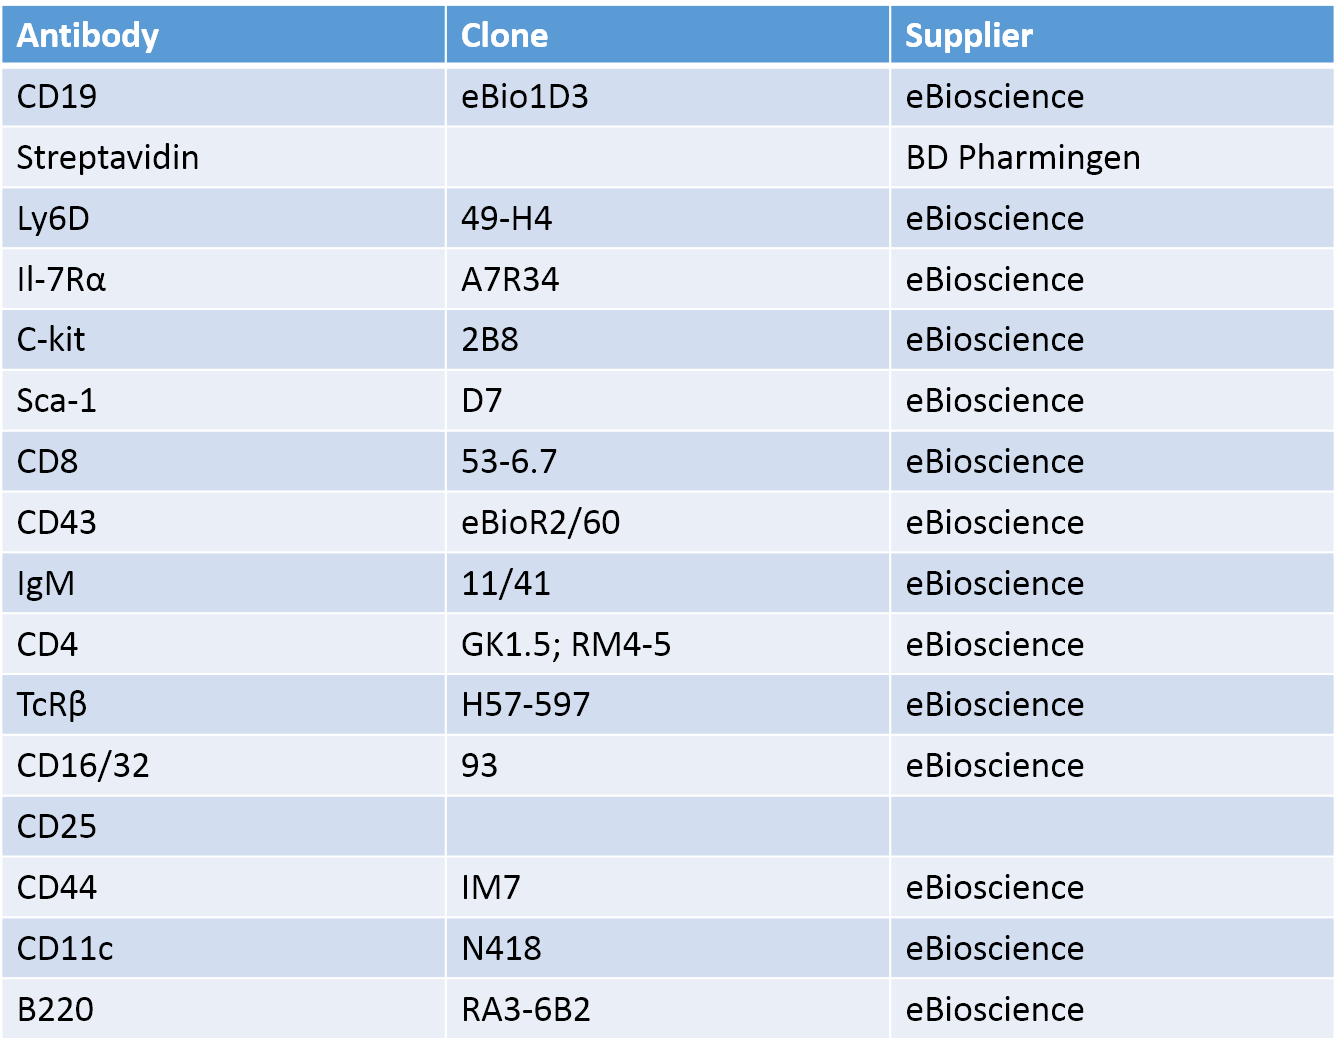
\includegraphics[width=\textwidth]{Figures/Antibodyclones.png}
\caption{Antibody clones and suppliers}
\label{fig:antibodyclones}
\end{table}

\section{Magnetic cell sorting}
\label{Methods:MACSdepletion}

\subsection{Miltenyi beads and columns}

Cells prepared as in \cref{sec:cellprep}.
For lineage depletion, lineage cell depletion kit (Miltenyi Biotech) was used.
For separation of samples into CD19\textsuperscript{+} and CD19\textsuperscript{-} fractions, CD19 microbeads (Miltenyi Biotech) were used.
For both lineage depletion and CD19 separation, Miltenyi LS columns were used and the maufacturers protocols were followed.
There were two deviations from the manufacturers protocol.
Firstly, the addition of an Fc receptor-blocking step prior to the addition of the beads using anti-CD16/32 antibody at 1:300 dilution.
Secondly, the buffer used was 0.5\% PBS/BSA, rather than the buffer suggested in the protocol.

\subsection{Qiagen BioMag goat anti-rat IgG beads}

Cells were prepared as in \cref{sec:cellprep}, resuspended in 500 $\mu$L of 0.5\% PBS/BSA.
A 1:300 dilution of anti-CD16/32 antibody was added and samples were incubated at 4 \textdegree C for 10 minutes to block Fc receptors.
Samples were then stained with appropriate purified antibody (See \toref{Antibody table}) and incubated for 20 minutes at 4 \textdegree C.
1 mL BioMag goat anti-rat IgG beads (Qiagen) taken and 10 mL PBS added.
Beads put on magnet and left for ~10 minutes to allow all beads to adhere.
Pasteur pipette used to remove and discard supernatant and beads resuspended in 500 $\mu$L of PBS.
Beads put back on magnet and beads allowed to adhere again before removing supernatant as before.
A final wash in 500 $\mu$L PBS performed then beads finally resuspended in 500 $\mu$L PBS.

Cells washed in 3 mL PBS and then centrifuged for 10 minutes at 1200 rpm.
Cells then resuspended in the washed beads and incubated for 15 minutes at 4 \textdegree C.

Samples then put on magnet and beads allowed to adhere.
Supernatant removed with clean pasteur pipette, kept, and put back on magnet to remove residual beads.
Supernatant obtained as before and kept as depleted sample.
If to be used for flow cytometry, samples centrifuged for 3 minutes at 1200 rpm, supernatant discarded then resuspended in an appropriate volume.

\section{RNA preparation}

Cells were prepared as in \cref{sec:cellprep}, then RNA extracted using RNeasy mini kits (Qiagen) following the maunufacturers protocol.
A DNAse step was included where Deoxyribonuclease I (Sigma) was added to column membrane for 10 minutes at room temperature.
The addition of a DNAse step improved the clarity of bands of products on gel electrophoresis following PCR by removing residual genomic DNA.
RNA quality was tested on the NanoDrop (ThermoScientific NanoDrop 2000), with the aim of producing RNA with 260/280 and 260/230 values of near to, or above, 2.0 which indicates a good purity of RNA.
RNA was stored at -80 \textdegree C.


\section{Reverse transcription of RNA to cDNA}

RNA was reverse transcribed to cDNA using Superscript II reverse transcriptase (Invitrogen).
RNA was taken and heated at 55 \textdegree C for 10 minutes before being placed on ice.
7 $\mu$L of first buffer (4 $\mu$L 5 x 1st strand buffer, 2 $\mu$L 10mM dNTPs, 1 $\mu$L OligodT 0.5 $\mu$LM) was added to 10 $\mu$L of RNA in RNAse-free PCR strips.
Amount of RNA was normalised across samples using data from NanoDrop in order to try and keep quantities of cDNA constant across samples.
RNA then made up to 10 $\mu$L with RNAse-free water.
Samples then incubated at 65 \textdegree C for 5 minutes.
3 $\mu$L of second buffer (1 $\mu$L 0.1M DTT, 1 $\mu$L RNAse out, 1 $\mu$L Superscript II) was then added to each sample then samples were incubated at 65 \textdegree C for 45-60 minutes to make cDNA.
cDNA stored at -20 \textdegree C until needed.

\section{Primer design}

Specific primers for polymerase chain reaction (PCR) to look for B cell development genes were designed by finding gene sequences in the NCBI nucleotide database \citep{NCBIdatabase} then looking for suitable primers for these genes using Primer3 \citep{Primer3}.
The primers were then put through a primer blast \citep{Primerblast} to check for specificiy and to find out any unintended targets.
Designed primers (obtained from Sigma Genosys) were then tested to find their optimum annealing temperature by carrying out a temperature gradient PCR from 52-62 \textdegree C.
This also checked that all primers were working, shown by a band at the expected product size when PCR products were run on a gel.

Primers are as follows:
\begin{itemize}
\item E2A. Forward TTG ACC CTA GCC GGA CAT AC.
Reverse TGC CAA CAC TGG TGT CTC TC.
Expected product size: 150bp.
Optimum annealing temperature: 61.8 \textdegree C.

\item EBF.
Forward CAG TTC TGC AAA GGG ACA CC.
Reverse CAA TGT CGG CAG CTC TCT TC.
Expected product size:226 bp.
Optimum annealing temperature: 59.4 \textdegree C.

\item Pax5. Forward AAC TTG CCC ATC AAG GTG TC.
Reverse CTG ATC TCC CAG GCA AAC AT.
Expected product size: 217bp.
Optimum annealing temperature 61.3 \textdegree C.

\item VPreB.
Forward CGA TAT CCC ACC TCG CTT CT.
Reverse CCG AGC AAA GCA AAC TCT GT.
Expected product size: 238 bp.
Optimum annealing temperature: 59.4 \textdegree C.

\item CXCL12.
Forward GCT CTG CAT CAG TGA CGG TA.
Reverse TAA TTT CGG GTC AAT GCA CA.
Expected product size: 184 bp.
Optimum annealing temperature: 60.5 \textdegree C.
\end{itemize}

\section{Polymerase chain reaction}

Polymerase chain reaction (PCR) was carried out to look for the genes of interest using the primers outlined above.
PCR samples consisted of 1 $\mu$L cDNA, 1.125 $\mu$L forward primer, 1.125 $\mu$L reverse primer, 2.5 $\mu$L MgCl{2} (Applied Biosystems), 2.5 $\mu$L MgCl{2} buffer (Applied Biosystems), 15.5 $\mu$L dH{2}O, 0.125 $\mu$L Taq Polymerase (Applied Biosystems).
PCRs were carried out using a 52-62 \textdegree C temperature gradient.

\section{Gel electrophoresis}

Gel electrophoresis of PCR products were carried out using 3\% agarose gels (Lonza SeaKem LE Agarose) made in 1 x Tris acetate-EDTA (TAE) buffer (Sigma) supplemented with 1 $\mu$L of 10 mg/mL ethidium bromide (\todo{EtBr supplier}) per 25 mL TAE buffer.
5 $\mu$L of 6x loading dye \todo{Supplier loading dye} were added to each 25 $\mu$L PCR product sample.
Total volume of 30 $\mu$L was then transferred to wells in the gel, held in a gel rig containing 1 x TAE buffer.
100 base pair (bp) ladder also put in a well of the gel to show size of bands seen in the gel.
Gels were run at constant 70 V until bands had separated sufficiently and imaged using SynGene software.

\section{Statistical Analyses}

All graphs were drawn using GraphPad Prism and statistical analyses (One way ANOVA, Tukey's tests and Mann-Whitney tests) were performed using built-in functions within the software.
